\documentclass[UTF8,AutoFakeBold,twoside]{XJTUMCM}

% ++++++++++++  文章排版设置  ++++++++++++ %
% ----------  调整页眉页脚样式  ---------- %
\usepackage{fancyhdr}
\pagestyle{fancy}
\fancyhf{}
\setlength{\headheight}{20pt}           % 设置页眉高度
\renewcommand{\headrulewidth}{0mm}      % 设置页眉线
\renewcommand{\footrulewidth}{0mm}      % 设置页脚线
% L-R: 左右
% E-O: 奇偶
% \fancyhead[RO]{\leftmark}
% \fancyhead[LE]{\titlecontent}
% \fancyhead[CO, CE]{\titlecontent}
% \fancyfoot[RO, LE]{\thepage}
\fancyfoot[C]{\thepage}

% -------------  行间距设置  ------------- %
\usepackage[nodisplayskipstretch]{setspace}
\setstretch{1.25}  % 全文行间距
\renewcommand{\captionfont}{\linespread{1}} % 题注行间距
\renewcommand{\arraystretch}{1.2}           % 表格行间距

% ------------  可选文章设置  ------------ %
% \usepackage{pdfpages}   % 国赛前两页最好用官方的word导出pdf插入比较好
\usepackage{blindtext}    % 生成无用文本看效果,没用
% \usepackage{sty/matlab} % 自定义的matlab语言关键词,代码高亮用
\usepackage{longtable}    % 跨页长表格
\usepackage{tabularx}     % 表格与页同宽所需环境
\usepackage{booktabs}     % 做三线表会比较需要
\usepackage{subcaption}   % 子图
\usepackage{inconsolata}  % linux等宽字体


% ++++++++++++  此处更改标题  ++++++++++++ %
\title{XJTU数模国赛模板}


\begin{document}
\bibliographystyle{gbt7714-numerical}
\nocite{*}  % 为了使所有参考文献加载出来。如果在文中已经用\cite标注出文献
            % 并且不需要所有参考文献都加载出来,则注释掉这一行
\maketitle
\begin{abstract}[keyword1][keyword2]
    abstract content
\end{abstract} % 引入摘要内容

% ++++++++++++  此处更改内容  ++++++++++++ %
\section{样式测试}
\subsection{二级标题}
\subsubsection{三级标题}
正文内容。正文内容正常撰写即可。
默认回车不会分段。

如果需要分段,则需要空一行。

\subsection{中英文测试}
\subsubsection{英文测试}
\blindtext[2]

\subsubsection{中文测试}
这是中文内容测试。

此开卷第一回也。作者自云:因曾历过一番梦幻之后,故将真事隐去,而借"通灵"之说,撰此《石头记》一书也。故曰"甄士隐"云云。但书所记何事何人?自又云:“今风尘碌碌,一事无成,忽念及当日所有之女子,一一细考较去,觉其行止见识,皆出于我之上。何我堂堂须眉,诚不若彼裙钗哉?实愧则有余,悔又无益之大无可如何之日也!当此,则自欲将已往所赖天恩祖德,锦衣纨绔之时,饫甘餍肥之日,背父兄教育之恩,负师友规谈之德,以至今日一技无成,半生潦倒之罪,编述一集,以告天下人:我之罪固不免,然闺阁本自历历有人,万不可因我之不肖,自护己短,一并使其泯灭也。虽今日之茅椽蓬牖,瓦灶绳床,其晨夕风露,阶柳庭花,亦未有妨我之襟怀笔墨者。虽我未学,下笔无,又何妨用假语村言,敷演出一段故事来,亦可使闺阁昭传,复可悦世之目,破人愁闷,不亦宜乎?故曰“贾雨村”云云。

此回凡用“梦”用“幻”等字,是提醒阅者眼目,亦是此书立意本旨。

列位看官:你道此书从何而来?说起根由虽近荒唐,细按则深有趣味。待在下将此来历注明,方使阅者了然不惑。

\section{图表环境}
\subsection{图片}
普通图片如\autoref{fig:sample}
\begin{figure}[H]
    \centering
    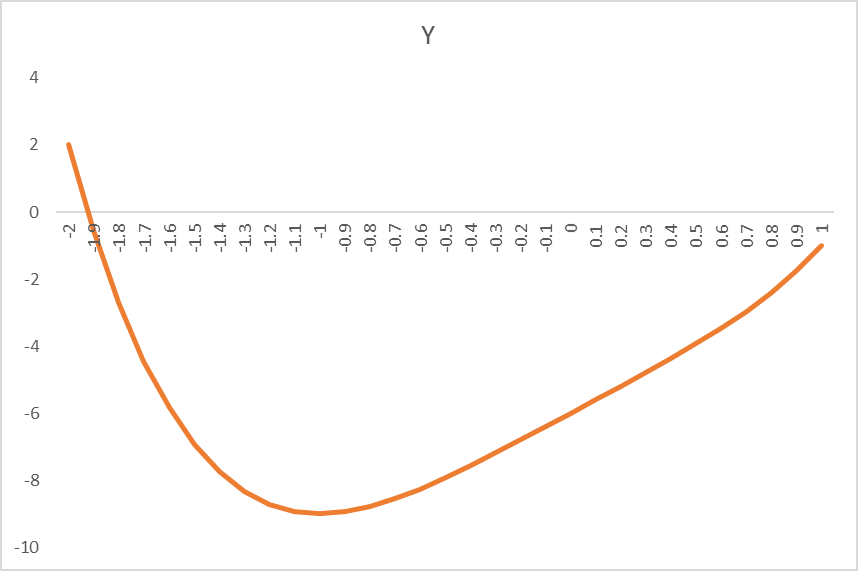
\includegraphics[width=8cm]{sample1.png}
    \caption{Sample Image}
    \label{fig:sample}
\end{figure}

子图环境如\autoref{fig:subfigure},也可以交叉引用子图,如\autoref{fig:subfig_b}

\begin{figure}[H]
    \begin{subfigure}{0.24\linewidth}
        
\includegraphics[width=\textwidth]{a.png}
        \caption{A字母图片}
    \end{subfigure}
    \hfill
    \begin{subfigure}{0.24\linewidth}
        
\includegraphics[width=\textwidth]{b.png}
        \caption{B字母图片}
        \label{fig:subfig_b}
    \end{subfigure}
    \hfill
    \begin{subfigure}{0.24\linewidth}
        
\includegraphics[width=\textwidth]{c.png}
        \caption{C字母图片}
    \end{subfigure}
    \hfill
    \begin{subfigure}{0.24\linewidth}
        
\includegraphics[width=\textwidth]{d.png}
        \caption{D字母图片}
    \end{subfigure}
    \caption{子图示例}
    \label{fig:subfigure}
\end{figure}

\subsection{表格}
\subsubsection{普通表格}
\begin{table}[htbp]
    \centering
    \caption{示例表格}
    \begin{tabular}{rlcc}
        \toprule
        ID & 名称        & 数量 & 单价 \\
        \midrule
        9  & Ruler       & 3    & 1000 \\
        26 & Pen         & 6    & 2000 \\
        32 & \LaTeX Book & 30   & 500  \\
        \bottomrule
    \end{tabular}
    \label{tab:}
\end{table}

\subsubsection{页宽表格}
\begin{table}[!ht]
    \caption{Parameter values}\label{tab:parametervalues}
    \begin{tabular*}{\hsize}{@{}@{\extracolsep{\fill}}ccccccccc@{}}
        \toprule
        &$p_{t}$  &21  &22  &20  &15  &10  &8   &  \\
        \midrule
        &$c_{t}$  &5   &13  &10  &10  &10  &10  &  \\
        &$h_{t}$  &10  &5   &5   &5   &5   &5   &  \\
        &$s_{t}$  &100 &100 &100 &100 &100 &100 &  \\
        &$d_{t}$  &30  &45  &50  &55  &45  &55  &  \\
        \bottomrule
    \end{tabular*}
\end{table}

\autoref{tab:parametervalues}左右都有多余的一列,这样内容能稍微紧凑好看一点。不然的话就是\autoref{tab:parametervalues_}这样

\begin{table}[!ht]
    \caption{Parameter values}\label{tab:parametervalues_}
    \begin{tabular*}{\hsize}{@{}@{\extracolsep{\fill}}ccccccc@{}}
        \toprule
        $p_{t}$  &21  &22  &20  &15  &10  &8     \\
        \midrule
        $c_{t}$  &5   &13  &10  &10  &10  &10    \\
        $h_{t}$  &10  &5   &5   &5   &5   &5     \\
        $s_{t}$  &100 &100 &100 &100 &100 &100   \\
        $d_{t}$  &30  &45  &50  &55  &45  &55    \\
        \bottomrule
    \end{tabular*}
\end{table}

\subsubsection{长表格}

\begin{longtable}{ccccccc}
    \caption{Longtable Caption Here.}                              \\

    \toprule
    ID & Name     & Chinese & Math & English & Physics & Chemistry \\
    \midrule
    \endfirsthead

    \multicolumn{7}{l}{\zihao{6}续上表}                            \\
    \toprule
    ID & Name     & Chinese & Math & English & Physics & Chemistry \\
    \midrule
    \endhead

    \bottomrule
    \multicolumn{7}{r}{\zihao{6}接下表}                            \\
    \endfoot

    \bottomrule
    \endlastfoot
    01 & Percival & 77      & 92   & 92      & 80      & 79        \\
    02 & Ida      & 74      & 87   & 99      & 96      & 73        \\
    03 & Janice   & 71      & 86   & 80      & 99      & 94        \\
    04 & Victor   & 82      & 60   & 100     & 63      & 67        \\
    05 & Oscar    & 61      & 86   & 89      & 100     & 77        \\
    06 & Janice   & 75      & 73   & 86      & 89      & 90        \\
    07 & Lulu     & 90      & 80   & 81      & 63      & 91        \\
\end{longtable}

\subsubsection{表格中含有图片}

\begin{table}[!ht]
    \centering
    \caption{table captoin here.}
    \begin{tabular}{ccc}
        \toprule
        Index    & Fig.A & Fig.B \\
        \midrule
        Pictures &
        \begin{minipage}[b]{0.12\columnwidth}
            \centering
            \raisebox{-0.5\height}{
\includegraphics[width=\linewidth]{a.png}}
        \end{minipage}
                 &
        \begin{minipage}[b]{0.12\columnwidth}
            \centering
            \raisebox{-0.5\height}{
\includegraphics[width=\linewidth]{b.png}}
        \end{minipage}
        \\
        \bottomrule
    \end{tabular}
\end{table}

\subsubsection{表格过宽}
表格过宽的第一反应一定是:这个表的形式是否正确,这个表放在这里是否真的有必要。如果确实有必要再用如下方法调整其宽度。

\begin{table}[!ht]
    \centering
    \caption{过宽表格}
    \resizebox{\linewidth}{!}{
        \begin{tabular}{ccc}
            \toprule
            变量              & 单位 & 描述                                                                                   \\
            \midrule
            $l_\textup{very}$ & m    & 这是一个很长很长很长很长很长很长很长很长很长很长很长很长很长很长很长很长很长很长的变量 \\
            \bottomrule
        \end{tabular}
    }
    \label{tab:toowide}
\end{table}

\subsubsection{过宽长表格}
这种更极端,更要首先考虑是否有必要。附录里放数据用用还可以。

思路:longtable是不兼容resizebox的,所以只能调小字号,使得宽度合适
{
\zihao{-6}
% \resizebox{\linewidth}{!}{
\begin{longtable}{clc ccc ccc ccc cc}
    \caption{6月部分小区二手房详细数据}                                                                                                               \\
    \hline
    行政区     & 小区名称     & 编号 & 建筑年龄 & 建筑面积 & 装修    & 绿化率  & 容积率  & 物业费  & 停车位  & 地铁数  & 购物中心 & 学校    & 医院    \\
    \hline
    \endfirsthead
    \multicolumn{14}{l}{\zihao{7}续上表}                                                                                                              \\
    \hline
    行政区     & 小区名称     & 编号 & 建筑年龄 & 建筑面积 & 装修    & 绿化率  & 容积率  & 物业费  & 停车位  & 地铁数  & 购物中心 & 学校    & 医院    \\
    \hline
    \endhead
    \hline
    \multicolumn{14}{r}{\zihao{7}接下表}                                                                                                              \\
    \endfoot
    \hline
    \endlastfoot

    未央区     & 恒大名都     & 1    & -0.4175  & 0.7360   & 0.4137  & 1.0222  & -0.047  & -0.1416 & -0.3166 & 0.4048  & -0.2817  & 0.8421  & 1.2480  \\
               & 华宇时间城   & 2    & -0.62    & -0.0419  & -1.5722 & -0.478  & -0.1422 & -0.1416 & 0.4742  & -1.3096 & 0.6402   & 0.0443  & -1.1705 \\
               & 西派国际     & 3    & -1.0249  & -0.3269  & -3.5582 & -0.478  & 0.3266  & 3.6994  & 0.0788  & -0.1667 & 0.0256   & 0.3102  & 0.6899  \\
               & 金桥太阳岛   & 4    & 1.6069   & -0.0276  & 0.4137  & 0.2721  & 0.0336  & -0.1416 & -0.3166 & 0.4048  & -1.8183  & 0.5762  & 0.8760  \\
    雁塔区     & 海伦国际     & 5    & -0.0127  & -0.1594  & -1.5722 & -0.478  & -0.5891 & 0.5058  & 0.4742  & 0.4048  & -1.2036  & 0.0443  & -0.0543 \\
               & 金裕花园     & 6    & 2.0118   & -1.3598  & 0.4137  & -2.7283 & 0.9127  & -0.789  & -0.712  & 0.4048  & -0.8963  & 0.5762  & 0.5039  \\
               & 豪盛时代华城 & 7    & 1.4044   & -1.4784  & 0.4137  & 1.0222  & 0.0336  & 0.5058  & -0.1848 & -0.7381 & -1.2036  & 1.108   & 1.2480  \\
               & 绿地与湖     & 8    & -0.8224  & -0.7383  & 0.4137  & -0.1779 & 0.7808  & 0.5058  & 1.1332  & -0.7381 & 0.9475   & 0.5762  & -1.7286 \\
\end{longtable}
}
% }
\section{公式}
\subsection{行内公式}
行内公式用两个\$包裹起来即可:

示例公式$E=mc^2$
\subsection{单行公式}
行间公式有多种写法,最常用的是equation,带编号,如\autoref{eq:eqsample}
\begin{equation}
    \sum_{i=1}^{n}\frac{1}{i}>\int_{1}^{n}\frac{1}{x}\d x=\ln(n+1)
    \label{eq:eqsample}
\end{equation}

如果公式不需要带编号,则可以简单的用一对\$\$括起来
$$
\int x^2 \d x = \frac{1}{3}x^3
$$

或者像这样
\begin{equation*}
    \int_{-\infty}^{+\infty}\delta(t)=1
\end{equation*}

\subsection{多行公式}
\subsubsection{align}
最常用align*。该环境下每行都会按照\&所在位置对齐。
\begin{align*}
    \int \frac{1}{x\ln x}\d x 
    &= \int \frac{1}{\ln x}\cdot \frac{1}{x}\d x\\
    &= \int \frac{1}{\ln x} \d \ln x\\
    &= \int  \d \ln((\ln x))\\
    &= \ln(\ln x)
\end{align*}

或者带编号,如\autoref{eq:alisample}
\begin{equation}
    \begin{aligned}
        a&=b\\
        c&=d
    \end{aligned}
    \label{eq:alisample}
\end{equation}

不使用align环境的原因是:align环境每一行都会有编号,使用较少。

大括号也是类似的方法生成的
$$
\varepsilon(t)=
\left\{
\begin{aligned}
    1&,t\ge 0\\
    0&,t<0
\end{aligned}
\right.
$$

\subsubsection{gather}
居中对齐环境
\begin{gather*}
    a+b=b+a\\
    a=b=c
\end{gather*}

\subsubsection{array}
array环境类似于表格,通常用于输出数组或更精细的公式排版
$$
\left(
    \begin{array}{cccc}
        a_{00}&a_{01}&a_{02}&a_{03}\\
        a_{10}&a_{11}&a_{12}&a_{13}\\
        a_{20}&a_{21}&a_{22}&a_{23}\\
        a_{30}&a_{31}&a_{32}&a_{33}\\
    \end{array}
\right)
$$
% 每一章节都在./page 下新建 .tex 文件并\include即可。
% 如果想每章节另起一页分页,可以将input改为include

\newpage
\bibliography{doc/bibfile}
\newpage
\begin{appendix}
    \section{代码}
    \lstinputlisting[
        style=python,
        breaklines=true,
        caption={python-sample}]{src/sample.py}
    \lstinputlisting[
        style=matlab,
        breaklines=true,
        caption={matlab-sample}]{src/sample.m}
\end{appendix}
\end{document}
